\chapter{自动控制系统的数学模型}
\thispagestyle{empty}
\noindent 建立数学模型的方法:
\begin{itemize}
	\item \dy[解析法]{JXF}:依据系统的及元件各个变量之间所遵循的物理、化学定律列写出变量间的数学表达式,并经实验验证。常用于简单的模型。
	\item \dy[实验法]{SYF}:对系统或元件输入一定形式的信号(如:阶跃信号、单位脉冲信号、正弦信号等),根据系统或元件的输出响应,经过数据处理而辨识出系统的数学模型。常用于复杂的模型。
\end{itemize}

\section{控制系统微分方程的建立}

\examples 弹簧-质量-阻尼器系统

\solve 分析质量$M$受力:
\begin{itemize}
	\item 外力:$r(t)$
	\item 弹簧恢复力:$Ky(t)$
	\item 阻尼力:$f \dfrac{\d y(t)}{\d t}$
\end{itemize}
根据牛顿第二定律,
\begin{equation*}
	m \frac{\d^2 y(t)}{\d t^2}=r(t)-f\frac{\d y(t)}{\d t}-K y(t)
\end{equation*}
即
\begin{equation}
	m \frac{\d^2 y(t)}{\d t^2} + f\frac{\d y(t)}{\d t} + K y(t) = r(t)
\end{equation}
令
\begin{equation*}
	T = \sqrt{\dfrac{m}{K}}, \quad 2\xi T = \frac fK \quad \Longrightarrow \xi = \frac{f}{2\sqrt{mK}}
\end{equation*}
则方程写为
\begin{equation*}
	T^2 \frac{\d^2 y(t)}{\d t^2} + 2\xi T\frac{\d y(t)}{\d t} + y(t) = \frac 1K r(t)
\end{equation*}
令$\omega_n=\dfrac 1 T$,则
\begin{equation}
	 \frac{\d^2 y(t)}{\d t^2} + 2\xi \omega_n\frac{\d y(t)}{\d t} + \omega_n^2y(t) = \frac {\omega_n^2}{K} r(t)
\end{equation}
其中,$T$称为时间常数,单位为s;$\xi$称为阻尼比,无量纲,$\omega_n$称为系统的无阻尼自然频率,单位为$\text{s}^{-1}$。

\newpage

\noindent 1. 列写微分方程的一般步骤
\begin{enumerate}[\hspace*{2em}(1)]
	\item 分析系统和各个元件的工作原理,找出各个物理量(变量)之间的关系,确定系统和各个元件的输入、输出变量。
	\item 从输入端开始,按照信号的传递顺序,根据各个变量所遵循的物理(或化学)定律,列写动态关系式,通常为1个微分方程组。
	\item 对已建立的微分方程组进行数学处理,忽略次要因素,简化原始方程,如对原始方程进行线性化等。
	\item 消除中间变量,写出关于输出、输入变量之间关系的数学表达式,即微分方程。
\end{enumerate}

\noindent 2. 线性系统

\defination[线性系统]
一般地,如下形式微分方程描述的系统称为\dy[线性系统]{XXXT}:
\begin{equation}
	\begin{split}
			a_0y^{(n)}&+a_1y^{(n-1)}+\cdots+a_{n-1}y'+a_ny\\
		&=b_0r^{(m)}+b_1r^{(m-1)}+\cdots+b_{m-1}r'+b_m r, \quad \quad m \le n
	\end{split}
\end{equation}
\noindent 其中,$r,y$关系如图\ref{线性系统}.
{
	\begin{center}
		\begin{tikzpicture}[node distance=1.2cm]
			%定义流程图具体形状
			\node(O) [minimum height=0cm,draw, node distance=1cm,inner sep=6pt] {线性系统};
			
			%连接具体形状
			\draw[arrows={-Stealth}](O) --+ (2cm,0)node[midway,right=0.8cm,above=-0.32cm]{{\large$y$}};
			\draw[arrows={-Stealth}](-2cm,0) -- (O)node[midway,right=-0.8cm,above=-0.24cm]{{\large$ r$}};

			%\draw[arrows={-Stealth}](A) --+(0,-1cm) node[midway,right=1.5cm,above=-0.3cm]{N}|-(A1) ;
			%\draw[arrows={-Stealth}](C) --+(0,-1.2cm)node[midway,right=2cm,above=-0.3cm]{取模函数mod}|-+(4cm,-1.2cm) -- (D1);
			%\draw[arrows={-Stealth}](C) --+(0,-1.2cm)node[midway,right=-2cm,above=-0.3cm]{取余函数rem}|-+(-4cm,-1.2cm) -- (D2);
		\end{tikzpicture}
		\captionof{figure}{线性系统}
		\label{线性系统}
	\end{center}
}
\noindent 若其所有系数均为常数,称为\dy[定常线性系统]{DCXXXT}:若至少有一个系统是时间的函数,则称为\dy[时变线性系统]{SBXXXT}。

\section{非线性微分方程的线性化}
在建立动态方程时会遇到元素的输入、输出变量之间具有非线性关系的情况。通常来说,构成系统的元件都具有不同的非线性程度。如图\ref{非线性}.
\begin{figure}[!htp]
	\centering
	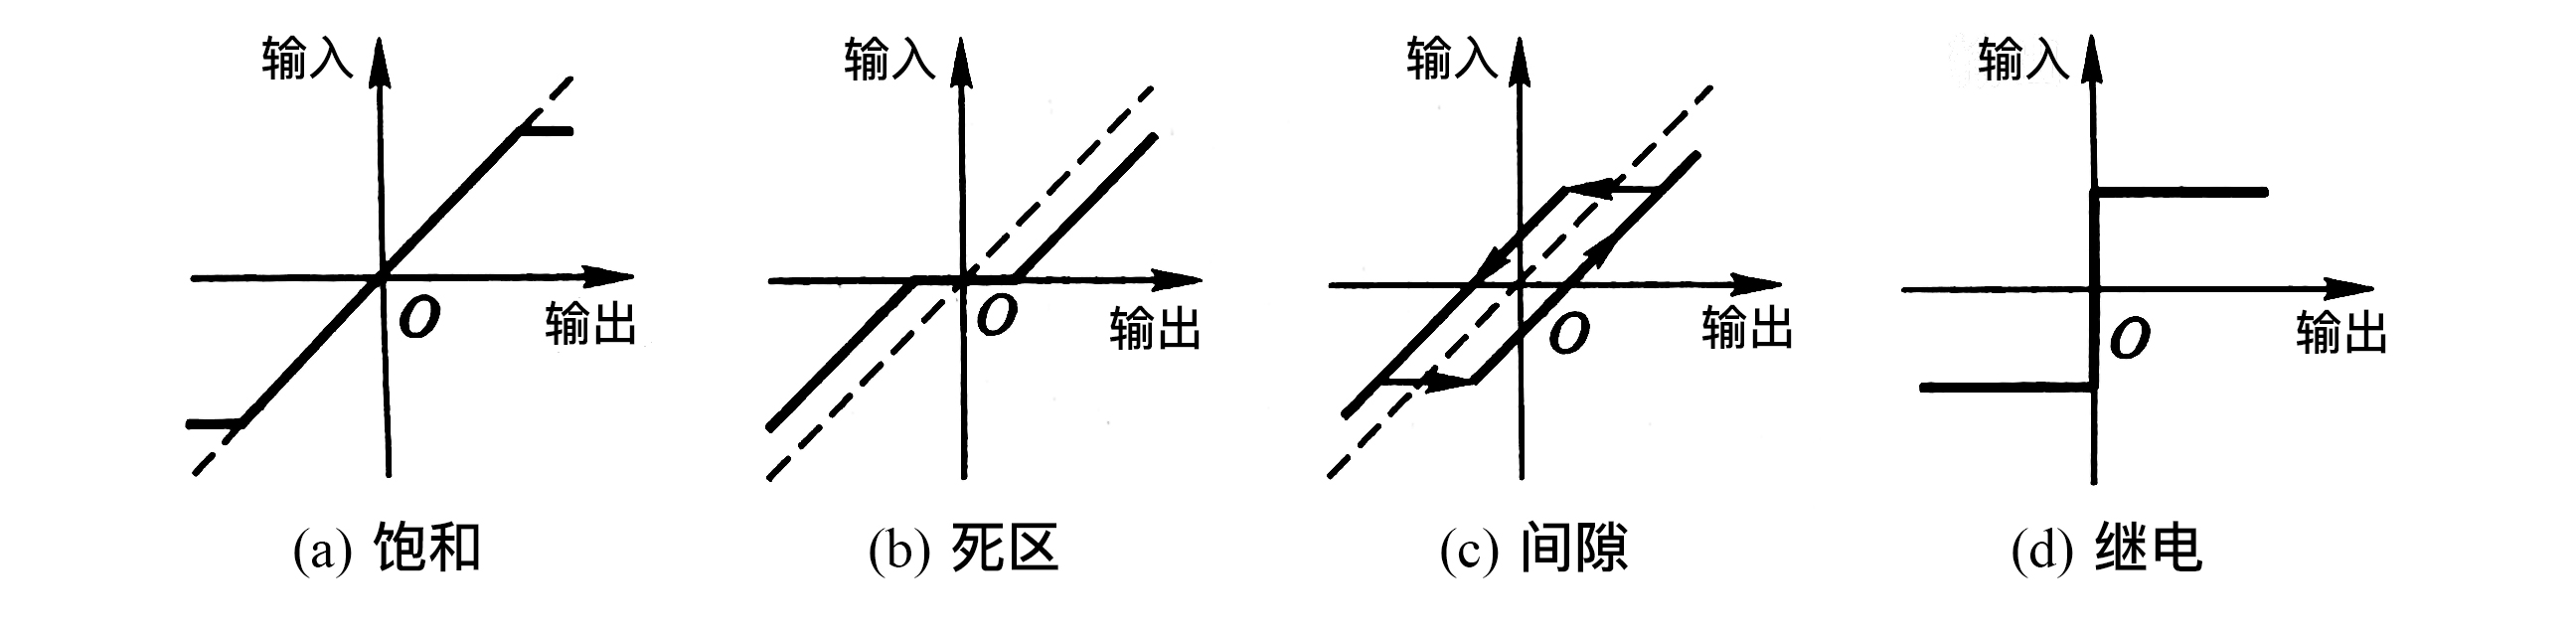
\includegraphics[width=0.95\linewidth]{pic/非线性.jpg}
	\caption{非线性特性}
	\label{非线性}
\end{figure}

\subsection{对弱非线性的线性化}
如图\ref{非线性}虚线所示,当输入信号很小时,忽略非线性影响,近似为放大特性。

\subsection{平衡位置附近的小偏差线性化}
输入、输出变量之间$y=f(x)$具有如图\ref{小偏差线性化}所示的非线性特性。
\begin{figure}[!htp]
	\centering
	
\includegraphics[width=0.5\linewidth]{pic/线性化.png}
	\caption{小偏差线性化}
	\label{小偏差线性化}
\end{figure}

当考虑到系统经常工作在平衡点$A(x_0,y_0)$处,当系统收到扰动后,变量$y$只在$A$点附近变化,这时表示系统在$A$点处的输出、输入关系函数可展成泰勒级数,即
\begin{equation}
	y = f(x) = f(x_0) + \left. \frac{\d f}{\d x} \right|_{x_0} \Delta x + \frac{1}{2!} \left. \frac{\d^2 f}{\d x^2}\right|_{x_0} \Delta x^2 + \cdots
	\label{线性化公式}
\end{equation}

式中:$\Delta x = x - x_0$,当$\Delta x$很小时,式\eqref{线性化公式}中$\Delta x^2$及高于$\Delta x^2$的项可以忽略,则得
\begin{equation}
	y=f(x)=f(x_0)+\left. \frac{\d f}{\d x}\right|_{x_0}\Delta x
	\label{线性公式2}
\end{equation}
记$\Delta y = f(x)- f(x_0)$,则由\eqref{线性公式2}可得
\begin{equation}
	\Delta y = \left. \frac{\d f}{\d x}\right|_{x_0}\Delta x
\end{equation}
式中$\displaystyle \left. \frac{\d f}{\d x}\right|_{x_0}\Delta x$为$\dfrac{\d f(x)}{\d x}$在$A$点处的值,代表了曲线$f(x)$在点$A$处的斜率。令$\left. \dfrac{\d f}{\d x}\right|_{x_0} = k$,则在$x_0$附近输出和输入的增量满足以下关系
\begin{equation}
	\Delta y = k \Delta x
	\label{线性公式3}
\end{equation}
显然,式\eqref{线性公式3}为$A$点处点切线方程,我们在平衡点$A$处用切线方程代替了非线性曲线方程$y=f(x)$,这就是小偏差线性化的几何意义。也可以写成
\begin{equation}
	y = kx
\end{equation}

\theorem[多元函数的小偏差线性化]
若非线性函数具有两个自变量$z=f(x,y)$,则在平衡点展成泰勒级数,忽略高次项,可简化为
\begin{equation}
	z = \left. \frac{\partial f}{\partial x} \right|_{(x_0,y_0)} x + \left. \frac{\partial f}{\partial y} \right|_{(x_0,y_0)} y
\end{equation}

\subsection{叠加原理}

叠加原理含有两重意义,即可叠加性和均匀性(或齐次性)。



\section{传递函数}
\subsection{传递函数的定义}
\tdefination[传递函数]
在零初始条件下,一个线性时不变系统输出的Laplace变换与输入的Laplace变换之比称为线性时不变的\dy[传递函数]{CDHS}。
\warn[
零初始条件
{
\begin{myitemize}
	\item 输入作用是在$t=0$之后才加于系统的,因此输入量及其各阶导数,在$t=0$时的值等于零。\vspace*{-0.5em}
	\item 输入信号作用于系统前是静止的,即$t=0$时,系统的输出量及各阶导数为零。\vspace*{0.3em}
\end{myitemize}
}
]
设任意系统的微分方程如下:
\begin{equation}
	\begin{split}
		&\quad a_0\frac{\d^n}{\d t^n}c(t) + a_1 \frac{\d^{n-1}}{\d t^{n-1}}c(t) + \cdots + a_{n-1}\frac{\d}{\d t}c(t)+a_nc(t)\\
		&=b_0\frac{\d^m}{\d t^m}r(t) + b_1 \frac{\d^{m-1}}{\d t^{m-1}}r(t) + \cdots + b_{m-1}\frac{\d}{\d t}r(t)+b_mr(t)
	\end{split}
\label{传递1}
\end{equation}
其中,$c(t)$为系统的输出,$r(t)$为系统的输入,$a_0,a_1,\cdots,a_n,b_0,b_1,\cdots,b_n$为与系统或元件结构、参数有关的常系数。

在初始条件为零时,对\eqref{传递1}两端取拉普拉斯变换,有
\begin{equation}
	\begin{split}
		&\quad \big(a_0s^n+a_1s^{n-1}+\cdots+a_{n-1}s+a_n\big)C(s)\\
		&\quad \big(b_0s^m+b_1s^{m-1}+\cdots+b_{m-1}s+b_m\big)R(s)
	\end{split}
\end{equation}
则
\begin{equation}
	\frac{C(s)}{R(s)}=G(s)=\frac{b_0s^m+b_1s^{m-1}+\cdots+b_{m-1}s+b_m}{a_0s^n+a_1s^{n-1}+\cdots+a_{n-1}s+a_n}=\frac{M(s)}{N(s)}
\end{equation}
其中,
\begin{equation*}
	\begin{split}
		&M(s) = b_0s^m+b_1s^{m-1}+\cdots+b_{m-1}s+b_m\\
		&N(s) = a_0s^n+a_1s^{n-1}+\cdots+a_{n-1}s+a_n
	\end{split}
\end{equation*}
\begin{myitemize}
	\item $M(s)$的根称为传递函数的零点,用$z_i, i =1,\cdots,m$表示。\vspace*{-0.5em}
	\item $N(s)$的根称为传递函数的极点,用$p_j, j =1, \cdots ,n$表示。\vspace*{0.3em}
\end{myitemize}

\subsection{传递函数的特点与说明}
\noindent 传递函数的优点:将动态系统的输入和输出关系用简单的代数方程来表示,如图\ref{传递函数}.
\begin{equation}
	Y(s) = G(s)X(s)
\end{equation}
{
	\begin{center}
		\begin{tikzpicture}[node distance=1.2cm]
			%定义流程图具体形状
			\node(O) [minimum height=0cm,draw=black!50,fill=black!20, node distance=1cm,inner sep=5pt] {$G(s)$};
			
			%连接具体形状
			\draw[arrows={-Stealth}](O) --+ (3cm,0)node[midway,right=1.7cm,above=-0.3cm]{{\large$y(t)$}};
			\draw[arrows={-Stealth}](-3cm,0) -- (O)node[midway,right=-1.7cm,above=-0.3cm]{{\large$x(t)$}};
			
		\end{tikzpicture}
		\captionof{figure}{传递函数}
		\label{传递函数}
	\end{center}
}

\noindent 关于传递函数,有以下几点说明:
\begin{myitemize}
	\item 1. 仅对LTI系统适用\vspace*{-0.5em}
	\item 2. 只反映系统的输入输出关系\vspace*{-0.5em}
	\item 3. 仅取决于系统的结构、参数,与输入形式无关\vspace*{-0.5em}
	\item 4. 不同的物理系统可以有相同的传递函数\vspace*{-0.5em}
	\item 5. 对真实的物理系统,有$m \le n.$\vspace*{0.3em}
\end{myitemize}


\section{系统的单位脉冲响应函数}
\subsection{单位脉冲响应}
当线性时不变系统输入单位脉冲信号,有
\begin{equation*}
	\begin{split}
		Y(s) &= G(s)R(s) = G(s)\mathcal{L}\big(\delta(t)\big)\\
		&=G(s)\cdot 1=G(s)
	\end{split}
\end{equation*}
因此
\begin{equation}
	y(t) = \mathcal{L}^{-1}\big[G(s)\big]=g(t)
\end{equation}

结论:\textbf{系统的传递函数的Laplace逆变换等于它的单位脉冲响应,即\dy[脉冲响应函数]{MCXYHS}}。

\noindent 对任意的系统,输入信号为$r(t)$,输出信号为$c(t)$,传递函数为$G(s)$,则
\begin{equation}
	C(s) = G(s)R(s)
\end{equation}
用Laplace变换的卷积定理可得:
\begin{equation}
	\begin{split}
		c(t) &= \mathcal{L}^{-1}\big[G(s)R(s)\big]\\
		& = g(t) * r(t)\\
		& = \int_0^t g(\tau)r(t-\tau) \,\d \tau
	\end{split}
\end{equation}

\example[利用卷积定理求输出响应]
给定
\[
Y(s) = G(s)R(s) = \frac{1}{s}R(s)
\]
若$R(s) = \dfrac{1}{s}$,求$y(t)$.

\solve
\begin{equation*}
	\begin{split}
		&g(t)=\mathcal{L}^{-1}\left(\frac{1}{s+1}\right)=\e^{-t},t \ge 0\\
		&r(t) = \mathcal{L}^{-1}\left(\frac{1}{s}\right)=1(t)
	\end{split}
\end{equation*}
故
\begin{equation*}
	y(t)=\int_0^t g(t-\tau)r(\tau)\,\d \tau=\int_0^t \e^{-(t-\tau)}\cdot 1\,\d \tau = 1 - \e^{-t},t \ge 0
\end{equation*}

\section{动态结构图}
\dy[动态结构图]{DTJGT}是表示组成控制系统的各个元件之间信号传递动态关系的图形。如图\ref{简单的动态结构图}.

{
	\begin{center}
		\begin{tikzpicture}[circuit ee IEC,node distance=1.2cm]
			%定义流程图具体形状
			\node[bulb] (A)  [minimum height=0cm,draw,below of = O, xshift = -2cm,node distance=1.5cm, inner sep=5pt,label=-80:$-$] {};
			\node (B) [minimum height=0cm,draw,below of = O, xshift = -0cm,node distance=1.5cm, inner sep=5pt] {$G(s)$};
			\node(O1) [minimum height=0cm,draw, below of = O, node distance=2.5cm,inner sep=5pt] {$H(s)$};
			
			%连接具体形状
			\draw[arrows={-Stealth}](O1) --+(-2cm,0) node[midway, right=-1.3cm, above=0cm]{$B(s)$} -- (A) ;
			\draw[arrows={-Stealth}](-3.5cm,-1.5cm) -- (A)  node[very near start,above=-3mm, xshift = -0.6cm]{$R(s)$};
			\draw[arrows={-Stealth}](A) -- (B) node[midway, above = 0.5mm]{$E$};
			\draw[arrows={-Stealth}](B) -- +(3cm,0) node[midway,above=-0.3cm,xshift = 18mm]{$C(s)$} ;
			\draw[arrows={-Stealth}](2cm,-1.5cm) --+(0,-1cm) -- (O1) ;
		\end{tikzpicture}
		\captionof{figure}{简单的动态结构图}
		\label{简单的动态结构图}
	\end{center}
}

\subsection{动态结构图的组成}
\noindent 控制系统的动态结构图一般由以下四种基本单元组成:

\begin{myitemize}
	\item \dy[信号线]{XHX}:带有箭头的直线,箭头表示信号传递的方向,信号线上标信号的原函数或象函数如图\ref{结构图1}.\vspace*{-0.5em}
	\item \dy[方框]{FK}:方框中为元部件的传递函数,它对信号起运算、转换作用,如图\ref{结构图2}.\vspace*{-0.5em}
	\item \dy[引出点]{YCD}(\dy[测量点]{CLD}):表示信号引出或测量位置,从同一点引出的信号完全相同,如图\ref{结构图3}.\vspace*{-0.5em}
	\item \dy[综合点]{ZHD}(\dy[比较点]{BJD}):对两个及以上的信号进行加减运算,"$+$"号表示相加,"$-$"表示相减,如图\ref{结构图4}.\vspace*{0.3em}
\end{myitemize}

\begin{figure}[!htb]
	\subfigure[信号线]{
	\begin{minipage}[b]{0.15\linewidth}
		\centering
		\begin{tikzpicture}[circuit ee IEC,node distance=1.2cm]
			\draw[arrows={-Stealth}](-0.75cm,-1cm)node[above=-1cm]{\quad} -- (0.75cm,-1cm) node[midway,  above=0cm]{$U(s)$} ;
		\end{tikzpicture}		
		\label{结构图1}
\end{minipage}
}
	\subfigure[方框]{
	\begin{minipage}[b]{0.25\linewidth}
		\centering
		\begin{tikzpicture}[node distance=1.2cm]
			%定义流程图具体形状
			\node(O) [minimum height=0cm,draw, node distance=1cm,inner sep=5pt] {$G(s)$};
			
			%连接具体形状
			\draw[arrows={-Stealth}](O) --+ (2cm,0)node[near end,above=0cm]{$C(s)$};
			\draw[arrows={-Stealth}](-2cm,0) -- (O)node[near start,above=0cm]{$U(s)$};
			
		\end{tikzpicture}
		\label{结构图2}
	\end{minipage}
}
	\subfigure[引出点]{
	\begin{minipage}[b]{0.2\linewidth}
		\centering
		\begin{tikzpicture}[circuit ee IEC,node distance=1.2cm]
			\draw[arrows={-Stealth}](-1cm,0)node[left = 0.1cm]{\quad} -- (1cm,0) node[near start,  above=0cm]{$U(s)$} ;
			\draw[arrows={-Stealth}](0cm,0) -- (0cm,-1.5cm) node[near end,  right=0.1cm]{$U(s)$} ;
		\end{tikzpicture}
		\label{结构图3}
	\end{minipage}
}
	\subfigure[综合点]{
	\begin{minipage}[b]{0.28\linewidth}
		\centering
		\begin{tikzpicture}[circuit ee IEC,node distance=1.2cm]
			\node[bulb] (A) [minimum height=0cm,draw, inner sep=5pt,label=-100:$\pm$] {};
			\draw[arrows={-Stealth}](-1.6cm,0) -- (A) node[near start,  above=0cm]{$\,\,U(s)$} ;
			\draw[arrows={-Stealth}](0cm,-1.2cm) -- (A) node[near start,  right=0.1cm]{$R(s)$} ;
			\draw[arrows={-Stealth}](A) -- (2.2cm,0) node[near end,  above=0cm]{$U(s)\pm R(s)$} ;
		\end{tikzpicture}
		\label{结构图4}
	\end{minipage}
}
\caption{动态结构图的四种基本组成单元}
\end{figure}

\subsection{结构动态图的等效变换}

\noindent 1. \textbf{串联方框连接及其等效变换}
\begin{figure}[!htb]
	\subfigure[]{
		\begin{minipage}[b]{0.5\linewidth}
			\centering
			\begin{tikzpicture}[circuit ee IEC,node distance=1.2cm]
				\node(A1) [minimum height=0cm,draw, node distance=1cm,inner sep=5pt] {$G_1(s)$};
				\node(A2) [minimum height=0cm,draw,right of= A1, node distance=2.5cm,inner sep=5pt,] {$G_2(s)$};
				\node(A3) [minimum height=0cm,draw,right of= A2, node distance=2.5cm,inner sep=5pt] {$G_n(s)$};
				
				\draw[arrows={-Stealth}](-1.5cm,0) -- (A1)node[midway ,above=0cm]{$R(s)$};
				\draw[arrows={-Stealth}](A1) -- (A2)node[midway ,above=0cm]{$U_1(s)$};
				\draw[arrows={-Stealth}](A2) -- (A3)node[midway ,above=0cm]{\large$\cdots$};
				\draw[arrows={-Stealth}](A3) --+(1.5cm,0)node[midway ,above=0cm]{$C(s)$};
			\end{tikzpicture}		
			\label{串联1}
		\end{minipage}
	}
	\subfigure[]{
		\begin{minipage}[b]{0.5\linewidth}
			\centering
			\begin{tikzpicture}[node distance=1.2cm]
				%定义流程图具体形状
				\node(O) [minimum height=0cm,draw, node distance=1cm,inner sep=5pt] {$G_1(s)G_2(s)\cdots G_n(s)$};
				
				%连接具体形状
				\draw[arrows={-Stealth}](-3cm,0) -- (O)node[midway, above=0cm]{$R(s)$};
				\draw[arrows={-Stealth}](O) --+ (3cm,0)node[midway, above=0cm]{$C(s)$};
				
			\end{tikzpicture}
			\label{串联2}
		\end{minipage}
	}
	\caption{串联方框连接及其等效变换}
\end{figure}


\noindent 2. \textbf{并联方框连接及其等效变换}
\begin{figure}[!htb]
	\centering
	\subfigure[]{
		\begin{minipage}[b]{0.4\linewidth}
			\centering
			\begin{tikzpicture}[circuit ee IEC,node distance=1.2cm]
				\node(A1) [minimum height=0cm,draw, node distance=1cm,inner sep=5pt] {$G_1(s)$};
				\node(A2) [minimum height=0cm,draw,below of= A1, node distance=1cm,inner sep=5pt] {$G_2(s)$};
				\node(A3) [minimum height=0cm,draw,below of= A2, node distance=1.3cm,inner sep=5pt,label=90:$\vdots$] {$G_n(s)$};
				\node[bulb] (C) [minimum height=0cm,draw,right of= A2, node distance=1.8cm,inner sep=5pt]{};

				
				\draw[arrows={-Stealth}](-2.5cm,-1cm) -- (A2);
				\draw[arrows={-Stealth}](-2.5cm,-1cm) -- (-1.5cm,-1cm)node[midway,above=0]{$R(s)$};
				\draw[arrows={-Stealth}](-2.5cm,-1cm) -- (-1.5cm,-1cm) -- (-1.5cm, 0cm) -- (A1);
				\draw[arrows={-Stealth}](-2.5cm,-1cm) -- (-1.5cm,-1cm) -- (-1.5cm, -2.3cm) -- (A3);
				\draw[arrows={-Stealth}](A1) --+(1.5cm,0) -- (C)node[near end,xshift=3mm]{$\pm$};
				\draw[arrows={-Stealth}](A3) --+(1.5cm,0) -- (C)node[near end,xshift=2mm]{$\pm$};
				\draw[arrows={-Stealth}](A2) -- (C)node[near end,above=0]{$\pm$};
				\draw[arrows={-Stealth}](C) --+(1cm,0)node[near end,above=-3mm,xshift=7mm]{$C(s)$};
				

			\end{tikzpicture}		
			\label{并联1}
		\end{minipage}
	}
	\subfigure[]{
		\begin{minipage}[b]{0.4\linewidth}
			\centering
			\begin{tikzpicture}[node distance=1.2cm]
				%定义流程图具体形状
				\node(O) [minimum height=0cm,draw, node distance=1cm,inner sep=5pt] {$G_1(s)\pm G_2(s)\pm \cdots \pm G_n(s)$};
				
				%连接具体形状
				\draw[arrows={-Stealth}](-3.2cm,0) -- (O)node[midway, above=0cm]{$R(s)$};
				\draw[arrows={-Stealth}](O)node[above=-1.62cm]{\quad} --+ (3.2cm,0)node[midway, above=0cm]{$C(s)$};
			\end{tikzpicture}
			\label{并联2}
		\end{minipage}
	}
	\caption{并联方框连接及其等效变换}
\end{figure}

\noindent 3. \textbf{引出点前后移动等效变换}
\begin{figure}[!htb]
	\centering
	\subfigure[引出点后移]{
	\begin{minipage}[b]{0.35 \linewidth}
		\centering
		\begin{tikzpicture}
			\node(A) [draw, inner sep = 6pt]{$G(s)$};
			
			\draw[arrows={-Stealth}](-2cm, 0cm) -- (A)node[near start, above = 0mm]{$R(s)$};
			\draw[arrows={-Stealth}](A) -- + (1.5cm,0cm)node[near end, above = 0mm]{$C(s)$};
			\draw[arrows={-Stealth}](-1.5cm,0cm) -- (-1.5cm,-1cm)node[midway, above= -10mm]{} -- (1.5cm,-1cm)node[very near end, above = 0mm]{$R(s)$};
		\end{tikzpicture}
	\end{minipage}
		\begin{minipage}[b]{0.35 \linewidth}
			\centering
		\begin{tikzpicture}
			\node(A) [draw, inner sep = 6pt]{$G(s)$};
			\node(B) [draw, inner sep = 2pt, right of = A,node distance = 2cm, yshift = -1cm]{$\,\,\dfrac{1}{G(s)}\,\,$};
			
			\draw[arrows={-Stealth}](-1.5cm, 0cm) -- (A)node[near start, above = 0mm]{$R(s)$} ;
			\draw[arrows={-Stealth}](A)-- + (3.5cm,0cm)node[very near end, above = 0mm]{$C(s)$};
			\draw[arrows={-Stealth}](1cm,0cm) -- (1cm,-1cm) --(B);
			\draw[arrows={-Stealth}](B) -- (3.5cm,-1cm)node[near end, above = 0mm]{$R(s)$};
		\end{tikzpicture}
	\end{minipage}
}
	\subfigure[引出点前移]{
	\begin{minipage}[b]{0.35 \linewidth}
		\centering
		\begin{tikzpicture}
			\node(A) [draw, inner sep = 6pt]{$G(s)$};
			
			\draw[arrows={-Stealth}](-1.5cm, 0cm) -- (A)node[near start, above = 0mm]{$R(s)$};
			\draw[arrows={-Stealth}](A) -- + (2cm,0cm)node[near end, above = 0mm]{$C(s)$};
			\draw[arrows={-Stealth}](1cm,0cm) -- (1cm,-1cm)node[midway, above= -10mm]{} -- (2cm,-1cm)node[near end, above = 0mm]{$C(s)$};
		\end{tikzpicture}
	\end{minipage}
	\begin{minipage}[b]{0.35 \linewidth}
		\centering
		\begin{tikzpicture}
			\node(A) [draw, inner sep = 6pt]{$G(s)$};
			\node(B) [draw, inner sep = 6pt, below of = A,node distance = 1cm]{$G(s)$};
			
			\draw[arrows={-Stealth}](-2cm, 0cm) -- (A)node[near start, above = 0mm]{$R(s)$};
			\draw[arrows={-Stealth}](A) -- + (2cm,0cm)node[very near end, above = 0mm]{$C(s)$};
			\draw[arrows={-Stealth}](-1cm, 0cm) -- (-1cm, -1cm) --(B);
			\draw[arrows={-Stealth}](B) -- (2cm,-1cm)node[very near end, above = 0mm]{$C(s)$};
		\end{tikzpicture}
	\end{minipage}
}
\caption{引出点前后移动变换等效}
\end{figure}


\noindent 4. \textbf{相邻引出点之间的移动}
\begin{myitemize}
	\item 相邻引出点之间互换位置是相互等效的。
	\vspace*{0.3em}
\end{myitemize}
\vspace*{0.5em}
\noindent 5. \textbf{综合点前后移动等效变换}
\begin{figure}[!htb]
	\centering
	\subfigure[综合点后移]{
		\begin{minipage}[b]{0.35 \linewidth}
			\centering
			\begin{tikzpicture}[circuit ee IEC]
				\node(A) [draw, inner sep = 6pt]{$G(s)$};
				\node[bulb] (O) [draw, inner sep = 5pt, left of = A, node distance = 1.5cm, label = -95:$\pm$,]{};
				
				\draw[arrows={-Stealth}](-2.5cm, 0cm) --(O)node[near start, above = 0mm]{$R(s)$};
				\draw[arrows={-Stealth}](O) -- (A);
				\draw[arrows={-Stealth}](A) -- + (1.5cm,0cm)node[near end, above = 0mm]{$C(s)$};
				\draw[arrows={-Stealth}](-1.5cm,-1.5cm)node[yshift = 0.2cm, xshift = 0.5cm]{$U(s)$} -- (O)node[midway, above= -6mm]{};
			\end{tikzpicture}
		\end{minipage}
		\begin{minipage}[b]{0.35 \linewidth}
			\centering
			\begin{tikzpicture}[circuit ee IEC]
				\node(A) [draw, inner sep = 6pt]{$G(s)$};
				\node(B) [draw, inner sep = 6pt, below of = A,node distance = 1.2cm]{$G(s)$};
				\node[bulb] (O) [inner sep = 5pt, right of = A, node distance =15mm, label = -95:$\pm$]{};
				
				\draw[arrows={-Stealth}](-1.5cm, 0cm) -- (A)node[near start, above = 0mm]{$R(s)$};
				\draw[arrows={-Stealth}](A) --(O);
				\draw[arrows={-Stealth}](O) -- + (1cm,0cm)node[very near end, above = 0mm]{$C(s)$};
				\draw[arrows={-Stealth}](-1.5cm, -1.2cm) -- (B)node[near start, above = 0mm]{$U(s)$};
				\draw[arrows={-Stealth}](B) -- (1.5cm,-1.2cm) -- (O);
			\end{tikzpicture}
		\end{minipage}
	}
	\subfigure[综合点前移]{
		\begin{minipage}[b]{0.35 \linewidth}
			\centering
			\begin{tikzpicture}[circuit ee IEC]
				\node(A) [draw, inner sep = 6pt]{$G(s)$};
				\node[bulb] (O) [draw, inner sep = 5pt, right of = A, node distance =1.5cm, label = -95:$\pm$] {};
				
				\draw[arrows={-Stealth}](-1.5cm, 0cm) -- (A)node[near start, above = 0mm]{$R(s)$};
				\draw[arrows={-Stealth}](A) -- (O);
				\draw[arrows={-Stealth}](O) -- (2.5cm,0cm)node[near end, above = 0mm]{$C(s)$};
				\draw[arrows={-Stealth}](1.5cm,-1.6cm)node[yshift =0.2cm, xshift = 0.5 cm]{$U(s)$} -- (O);
			\end{tikzpicture}
		\end{minipage}
		\begin{minipage}[b]{0.35 \linewidth}
			\centering
			\begin{tikzpicture}[circuit ee IEC]
				\node(A) [draw, inner sep = 6pt]{$G(s)$};
				\node(B) [draw, inner sep = 2pt, below of = A,node distance = 1.2cm]{$\,\,\dfrac{1}{G(s)}\,\,$};
				\node[bulb] (O) [draw, inner sep =5pt, left of = A, node distance = 1.5cm, label = -85:$\pm$] {};
				
				\draw[arrows={-Stealth}](-2.5cm, 0cm) --(O)node[very near start, above = 0mm]{$R(s)$};
				\draw[arrows={-Stealth}](O) -- (A);
				\draw[arrows={-Stealth}](A) -- + (2cm,0cm)node[very near end, above = 0mm]{$C(s)$};
				\draw[arrows={-Stealth}](2cm, -1.2cm)  --(B)node[very near start, above = 0mm]{$U(s)$};
				\draw[arrows={-Stealth}](B) -- (-1.5cm,-1.2cm) -- (O);
			\end{tikzpicture}
		\end{minipage}
	}
	\caption{综合点前后移动变换等效}
\end{figure}


\noindent 6. \textbf{相邻综合点之间的移动}
\begin{myitemize}
	\item 相邻综合点之间互换位置是相互等效的,也可以把它们简化为一个综合点。
	\vspace*{0.3em}
\end{myitemize}
\vspace*{0.5em}

\noindent 7. \textbf{方框反馈连接及其等效变换}
\begin{figure}[!htb]
	\centering
	\subfigure[]{
		\centering
	\begin{minipage}[b]{0.35\linewidth}
		\begin{tikzpicture}[circuit ee IEC]
			\node(A) [draw, inner sep =6pt]{$G(s)$};
			\node(B) [draw, inner sep =6pt, below of = A, node distance = 1cm]{$H(s)$};
			\node[bulb] (O) [draw, inner sep =5pt, left of = A, node distance = 2cm, label = -95:$\pm$]{};
			
			\draw[arrows={-Stealth}](-3cm, 0) -- (O)node[near start, above = 0mm]{$R(s)$};
			\draw[arrows={-Stealth}](O) -- (A)node[midway, above = 0mm]{$E(s)$};
			\draw[arrows={-Stealth}](A) -- (2cm, 0cm)node[midway, above = 0mm,xshift = 5mm]{$C(s)$};
			\draw[arrows={-Stealth}](1.5cm, 0cm) -- +(0cm, -1cm) -- (B);
			\draw[arrows={-Stealth}](B) -- (-2cm,-1cm) -- (O)node[midway, xshift =5mm,yshift =1mm]{$B(s)$};
		\end{tikzpicture}
	\end{minipage}	
}
\subfigure[]{
\centering
\begin{minipage}[b]{0.35\linewidth}
	\centering
	\begin{tikzpicture}
		\node(A) [draw,inner sep = 4pt]{$\,\,\dfrac{G(s)}{1 \mp G(s)H(s)}\,\,$};
		
		\draw[arrows={-Stealth}](-2cm, 0cm)node[yshift = -8mm]{} -- (A)node[near start, above = 0mm]{$R(s)$};
		\draw[arrows={-Stealth}](A) -- (2cm, 0cm) node[near end, above = 0mm]{$C(s)$};
	\end{tikzpicture}
\end{minipage}
}
\caption{方框反馈连接}
\end{figure}

\subsection{梅森公式}
\ttheorem[梅森公式]
\vspace*{-0.5em}
\begin{equation}
	G(s) = \frac{\displaystyle \sum_{k = 1}^{n}P_k\Delta_k}{\Delta}
\end{equation}
其中,
\begin{myitemize}
	\item $G(s)$为待求的传递函数
	\item $\Delta$ 为特征式
	\begin{itemize}
		\item 表达式:$\Delta  = 1 - \sum L_i + \sum L_iL_j - \sum L_iL_jL_k \cdots$
		\item $\sum L_i$:所有各回路的回路传递函数之和
		\item $L_iL_j$:两两互相不接触的回路的传递函数的乘积(含符号)
		\item $L_iL_jL_k$:3个互不接触回路的传递函数的乘积(含符号),以此类推……
	\end{itemize}
	\item $N$为\dy[前向通路]{QXTL}(从$R(s)$到$C(s)$且不重复访问同一点)的条数
	\item $P_k$为第$k$条前向通路传递函数的乘积
	\item $\Delta_k$为第$k$条前向通路的\dy[余子式]{YZS},即在$\Delta  = 1 - \sum L_i + \sum L_iL_j - \sum L_iL_jL_k \cdots$中去除与前向通路$P_k$接触的回路$L_k$后的余项。
\end{myitemize}

\section{典型反馈系统的几种传递函数}
\begin{figure}[!htb]
	\centering
		\centering
			\begin{tikzpicture}[circuit ee IEC]
				\node(A) [draw, inner sep =6pt]{$G_1(s)$};
				\node[bulb] (C) [draw, inner sep = 5pt, right of = A, node distance = 1.5cm, label = 95:$+$] {};
				\node (D) [draw, inner sep = 6pt, right of = C, node distance = 1.5cm]{$G_2(s)$};
				\node (B) [draw, inner sep =6pt, below of = C, node distance = 1.5cm]{$H(s)$};
				\node[bulb] (O) [draw, inner sep =5pt, left of = A, node distance = 2cm, label = -95:$-$]{};
				
				\draw[arrows={-Stealth}](-3cm, 0) -- (O)node[near start, above = 0mm]{$R(s)$};
				\draw[arrows={-Stealth}](O) -- (A)node[midway, above = 0mm]{$E(s)$};
				\draw[arrows={-Stealth}](A)-- (C);
				\draw[arrows={-Stealth}](C) -- (D);
				\draw[arrows={-Stealth}](D) -- +(1.5cm, 0cm)node[midway, above = 0mm,xshift = 5mm]{$C(s)$};
				\draw[arrows={-Stealth}](4cm, 0cm) -- +(0cm, -1.5cm) -- (B);
				\draw[arrows={-Stealth}](B) -- (-2cm,-1.5cm) -- (O)node[midway, xshift =5mm,yshift =1mm]{$B(s)$};
				\draw[arrows={-Stealth}](1.5cm, 1.5cm) -- (C)node[near start, xshift = 0.5cm]{$N(s)$};
			\end{tikzpicture}
	\caption{反馈系统的典型结构}
	\label{反馈典型}
\end{figure}

\subsection{系统的开环传递函数}
它是当主反馈回路断开时从$E(s)$到反馈信号$B(s)$之间的传递函数(不计符号)。\index{KHCDHS@开环传递函数}即
\begin{align}
	G(s) = G_1(s)G_2(s)H(s)
\end{align}

\subsection{输入信号下系统的闭环传递函数与误差传递函数}
令干扰信号$n(t) = 0$,则闭环传递函数为
\begin{align}
	\varPhi(s) = \dfrac{C(s)}{R(s)} = \dfrac{G_1(s)G_2(s)}{1 + G_1(s)G_2(s)H(s)}
\end{align}

\newpage

由图\ref{反馈典型}中将输入改为$R(s)$,输出改为$E(s)$,得到转换后的结构图如图\ref{输入误差}.
\begin{figure}[!htb]
	\centering
	\begin{tikzpicture}[circuit ee IEC]
		\node[bulb] (A) [draw, inner sep = 5pt, label = -95:$-$] {};
		\node (B) [draw, inner sep = 6pt, below of = A, xshift = 1.2cm, node distance = 1.5cm]{$H(s)$};
		\node (C) [draw, inner sep = 6pt, below of = A, xshift = 2.85cm, node distance = 1.5cm]{$G_1(s)$};
		\node (D) [draw, inner sep = 6pt, below of = A, xshift = 4.5cm, node distance = 1.5cm]{$G_2(s)$};
		
		\draw[arrows={-Stealth}](-1cm, 0cm) -- (A)node[near start, above = 0cm]{$R(s)$};
		\draw[arrows={-Stealth}](A) -- +(6.5cm, 0cm)node[very near end, above = 0cm]{$E(s)$};
		\draw[arrows={-Stealth}](5.75cm,0cm) -- +(0cm, -1.5cm) -- (D);
		\draw[arrows={-Stealth}](D) -- (C);
		\draw[arrows={-Stealth}](C) -- (B);
		\draw[arrows={-Stealth}](B) -- +(-1.2cm, 0cm) -- (A);
		
	\end{tikzpicture}
	\caption{输入误差结构图}
	\label{输入误差}
\end{figure}

由动态结构图的化简或梅森公式可得其误差函数为
\begin{align}
	E_r(s) =  \dfrac{R(s)}{1 + G_1(s)G_2(s)H(s)}
\end{align}

\noindent 所以误差传递函数为
\begin{align}
	\varPhi_{\text{er}}(s) = \dfrac{E(s)}{R(s)} = \dfrac{1}{1 + G_1(s)G_2(s)H(s)}
\end{align}

\subsection{干扰信号下系统的闭环传递函数与误差传递函数}
令输入信号$r(t) = 0$,则闭环传递函数为
\begin{align}
	\varPhi_n(s) = \dfrac{C(s)}{N(s)} = \dfrac{G_2(s)}{1 + G_1(s)G_2(s)H(s)}
\end{align}

由图\ref{反馈典型}中将输入改为$N(s)$,输出改为$E(s)$,得到转换后的结构图如图\ref{输入误差}.
\begin{figure}[!htb]
	\centering
	\begin{tikzpicture}[circuit ee IEC]
		\node[bulb] (A) [draw, inner sep = 5pt, label = -95:$+$] {};
		\node (B) [draw, inner sep = 6pt, right of = A, node distance = 1.5cm]{$G_2(s)$};
		\node (C) [draw, inner sep = 6pt, right of = B, node distance = 2cm]{$-H(s)$};
		\node (D) [draw, inner sep = 6pt, below of = B, xshift = 0.75cm, node distance = 1.5cm]{$G_1(s)$};
		
		\draw[arrows={-Stealth}](-1cm, 0cm) -- (A)node[near start, above = 0cm]{$R(s)$};
		\draw[arrows={-Stealth}](C) -- +(2cm, 0cm)node[very near end, above = 0cm]{$E(s)$};
		\draw[arrows={-Stealth}](4.75cm,0cm) -- +(0cm, -1.5cm) -- (D);
		\draw[arrows={-Stealth}](D) -- +(-2.25cm, 0cm) -- (A);
		\draw[arrows={-Stealth}](A) -- (B);
		\draw[arrows={-Stealth}](B) -- (C);
		
	\end{tikzpicture}
	\caption{干扰误差结构图}
	\label{干扰误差}
\end{figure}

由动态结构图的化简或梅森公式可得其误差函数为
\begin{align}
	E_n(s)  = \dfrac{-G_2(s)H(s)}{1 + G_1(s)G_2(s)H(s)}N(s)
\end{align}
所以误差传递函数为
\begin{align}
	\varPhi_{\text{en}}(s) = \dfrac{E(s)}{N(s)} = \dfrac{-G_2(s)H(s)}{1 + G_1(s)G_2(s)H(s)}
\end{align}

\vspace*{1em}
根据叠加定理,系统在$r(t)$和$n(t)$同时作用下的总输出为
\begin{align}
	C(s) = \varPhi(s)R(s) + \varPhi_n(s) N(s) = \dfrac{G_1(s)G_2(s)}{1 + G_1(s)G_2(s)H(s)}R(s) +  \dfrac{G_2(s)}{1 + G_1(s)G_2(s)H(s)} N(s)
\end{align}
系统的总误差为
\begin{align}
	E_\Sigma (s) = \dfrac{1}{1 + G_1(s)G_2(s)H(s)}R(s) + \dfrac{-G_2(s)H(s)}{1 + G_1(s)G_2(s)H(s)}N(s)
\end{align}










